\documentclass[a4paper, 11pt]{report}
%\usepackage[a4paper, lmargin={3cm}, rmargin={3cm}, tmargin={2.5cm}, bmargin={2.5cm} ]{geometry}

%+++ Packages +++++++++++++++++++++++++++++++++++++++++++++++++++++++++++++++++

%%%%% Math %%%%%
\usepackage{amsmath} 
\usepackage{amssymb}

\setlength{\parindent}{0pt} 
%%%%% Umlaute %%%%%
\usepackage[utf8]{inputenc}
%%%%% Hilft Latex bei Deutschen Wörtern (Linebreak, etc) %%%%%
\usepackage[german, english]{babel} 
%%%%% Grafiken %%%%%
\usepackage[pdftex]{graphicx}
\usepackage{epstopdf}
%%%%% Platziere Figure an einem bestimmten ort mit '[H]' %%%%%
\usepackage{float}
%%%%% Querformat für bilder %%%%%
\usepackage{rotating}
%%%%% url %%%%%
\usepackage{url}
%%%%% Klickbare Links im Inhaltsverzeichnis %%%%%
\usepackage{hyperref}
\hypersetup{pdfborder = {0 0 0}}
%%%%% Kommentare sind moeglich mit \begin{comment} %%%%%
\usepackage{comment}
%\pagestyle{plain}
\usepackage{a4}

%%%%% Source Code darstellen %%%%%
\usepackage{listings}
\lstset{basicstyle=\small\ttfamily, tabsize=4, numbers=left, numberstyle=\tiny, language=C++}
\lstset{literate=%
{Ö}{{\"O}}1 %
{Ä}{{\"A}}1 %
{Ü}{{\"U}}1
{ß}{{\ss}}2 %
{ü}{{\"u}}1 %
{ä}{{\"a}}1 %
{ö}{{\"o}}1 %
}
%\renewcommand\lstlistingname{Code}
%%%%% Grafiken mit Latex zeichnen %%%%%
\usepackage{tikz}
\usetikzlibrary{arrows}

%%%%% Bilder zentriert Ausrichten %%%%%
\usepackage[center]{caption}

%%%%% Tabellen %%%%%
\usepackage{setspace,booktabs}
\usepackage{tabu}

%+++ Dokument Styling +++++++++++++++++++++++++++++++++++++++++++++++++++++++++
\usepackage{geometry}
\geometry{a4paper, top=25mm, left=27mm, right=28mm, bottom=28mm, headsep=7mm, footskip=7mm}

\setlength{\headheight}{14pt}
%\renewcommand{\familydefault}{\rmfamily}

%\addtokomafont{caption}{\raggedright}

%+++ Kopf- und Fusszeilen +++++++++++++++++++++++++++++++++++++++++++++++++++++
\usepackage{fancyhdr}
\usepackage{lastpage}

\pagestyle{fancy}
\fancyhf{}
\fancyhead[L]{\leftmark}
\renewcommand{\sectionmark}[1]{\markboth{#1}{}}
%\cfoot{\thepage $ $ / \pageref{LastPage}} 
\cfoot{\small  \thepage} 

\renewcommand{\headrulewidth}{0.4pt} 

%+++ Leere Seiten -> keine Seitenzahlen +++++++++++++++++++++++++++++++++++++++
% redefinition of the plain style for Chapter:
\fancypagestyle{plain}{%
	\fancyhf{} % clear all header and footer fields
	\renewcommand{\headrulewidth}{0pt}
	\cfoot{\small  \thepage} 
}


%+++ thebibliography umbenennen +++++++++++++++++++++++++++++++++++++++++++++++
%\renewcommand{\refname}{Quellenangabe}

\def\BibTeX{{\rm B\kern-.05em{\sc i\kern-.025em b}\kern-.08em
    T\kern-.1667em\lower.7ex\hbox{E}\kern-.125emX}}
    
%\let\oldbibitem=\bibitem
%\renewcommand{\bibitem}[2][]{\oldbibitem[#1]{#2}\newline}

%++++++++++++++++++++++++++++++++++++++++++++++++++++++++++++++++++++++++++++++
%+++ Dokument Begin +++++++++++++++++++++++++++++++++++++++++++++++++++++++++++
%++++++++++++++++++++++++++++++++++++++++++++++++++++++++++++++++++++++++++++++
\begin{document}
%+++ Römische Seitenzahlen ++++++++++++++++++++++++++++++++++++++++++++++++++++
\pagenumbering{Roman} 

%+++ HTWG gemurkse ++++++++++++++++++++++++++++++++++++++++++++++++++++++++++++++++++
\newcommand{\thema}{Imagination-Augmented Agents for Deep Reinforcement Learning}
\newcommand{\schlagworte}{}

\newcommand{\zusammenfassung}{bla

\vspace*{0.3cm}

blub
}


\newcommand{\autor}{Angela Denninger}
\newcommand{\autorStrasse}{Hindenburgstr. 13}
\newcommand{\autorPLZ}{78467 }
\newcommand{\autorOrt}{Garching bei München}

\newcommand{\autorGeburtsort}{Tübingen}
\newcommand{\autorGeburtsdatum}{17.06.1990}

\newcommand{\supervisor}{Prof. Laura Leal-Taixé}
\newcommand{\advisor}{Tim Meinhardt}


\newpage
%+++ Title ++++++++++++++++++++++++++++++++++++++++++++++++++++++++++++++++++++

\begin{titlepage}

\vspace*{-1.5cm}
\begin{flushleft}
\hspace*{-1cm} 
\includegraphics[width=3.0cm]{Images/Universitaet_Logo_RGB}
\end{flushleft}

\vspace{2.5cm}

\begin{center}
	\huge{\textbf{\thema}} \\[1.5cm]

	\LARGE{\autor} \\[0.5cm]
	
	\large{Munich, 18.10.2018}\\[2.3cm]	
	
	\Large{Dynamic Vision and Learning Group}\\[1.5cm]
	
	\large{Supervisor: \supervisor}\\
	\large{Advisor: \advisor}
\end{center}

\vspace*{3.5cm}

%\begin{tabular}{p{3.4cm}p{10cm}}
%	Supervisor:    & \supervisor \\
%	Advisor:    & \advisor
%\end{tabular}


\end{titlepage}




%+++ Abstract +++++++++++++++++++++++++++++++++++++++++++++++++++++++++++++++++
\newpage
\section*{Abstract}

\vspace{5ex}

\noindent

bla



%+++ Inhaltsangabe umbenennen +++++++++++++++++++++++++++++++++++++++++++++++++
\renewcommand\contentsname{Inhaltsverzeichnis}
\tableofcontents
\renewcommand\partname{Kapitel}

%+++ figurename umbenennen ++++++++++++++++++++++++++++++++++++++++++++++++++++
%\renewcommand{\figurename}{Abbildung}

\chapter{I2A}
\section{Reinforcement learning}

Reinforcement Learning refers to a kind of Machine Learning method in which an agent learns to solve a given task by maximizing the received reward signal, where the agent represents the reinforcement learning algorithm.\\


\begin{figure}[H]
  \centering
  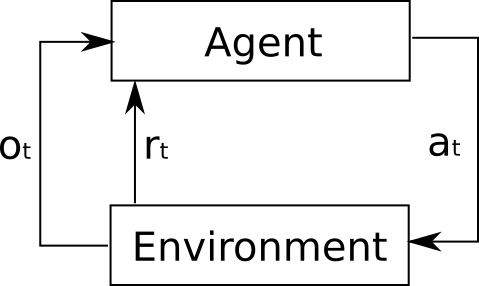
\includegraphics[width=300px]{Images/rl_agent.png} 
  \caption{Agent: reinforcement learning algorithm; Environment: object the agent is acting on; $a_t$: action the agent performes in the environment; $o_t$: observation (current state) of the environment the agent receives; $r_t$: reward signal the agent receives from the environment}
  \label{fig:reinforcement_learning}
\end{figure}


Figure \ref{fig:reinforcement_learning} shows the interaction of the agent with the environment, where the environment refers to the object the agent is acting on. As initial state the agent receives the observation $o_t$ of the environment at time $t = 0$. The observation $o_t$ can be the complete state of the environment, or just a subset of it.
The agent then, based on the observation $o_t$, performs an action $a_t$ in the environment, chosen from a set of possible actions (e.g. moving to the right or moving to the left). After performing the action $a_t$ the agent receives the new observation $o_{t+1}$ of the environment and also the reward signal $r_{t+1}$ which evaluates how good the chosen action was.
Based on the new information the agent again chooses an action $a_t$. The loop continues until the environment sends a termination state.\\

The goal of the agent is to maximize the received reward, which is done by learning an optimal action choosing function called policy, using the received reward signal.
There exist different reinforcement learning algorithms, which all follow the iterative learning algorithm described above, but differ in the update strategy for learning an optimal policy. In the following a short overview over different types of reinforcement learning algorithms will be given.\\

\subsection{Q-learning}

Q-learning is a reinforcement learning algorithm  introduced by Watkins \cite{QLearning} in 1989. 
For any finite markov decision process, Q-learning finds a policy that maximizes the expected total reward over all following steps, starting from the current state.
To do so Q-Learning learns a Q-table, which contains for each state-action pair $(s, a)$ a Q-value representing the expected future reward for taking the action $a$ in state $s$. 
By iteratively updating the Q-value function with the Bellman Equation, the Q-value function will converge to the optimal Q-value function \cite{QLearningProof}.\\

The Bellman Equation 

\begin{equation} \label{eq:bellman_eq1}
Q_{\pi} (s_t, a_t) =\mathbb{E}_{s_{t+1}} [r + \gamma Q_\pi(s_{t+1}, a_{t+1}) | s_t, a_t]
\end{equation}

states, that the Q-value for the state-action pair $(s_t, a_t)$ is equal to the expectation of the received reward $r$, of taking action $a$ in state $s$, plus the discounted future reward the agent will get by following the policy $\pi$ from the next state onwards, where $\gamma$ refers to the discount factor.\\


The optimal Q-value, denoted as $Q^* (s_t, a_t)$ can be expressed as:
\begin{equation} \label{eq:1}
Q^* (s_t, a_t) = \mathbb{E}_{s_{t+1}} [r + \gamma \max_{a_{t+1}} Q^*(s_{t+1}, a_{t+1}) | s_t, a_t]
\end{equation}

After the agent has converged to the optimal policy $Q^* (s_t, a_t)$ it is able to to choose in each possible state the optimal action.\\


\subsection{Value-based versus policy-based reinforcement learning methods}


Value-based methods are learning a value function, which maps state-action pairs directly to values. The best action in a certain state can then be found by taking the action with the biggest value. 
The policy is therefore the action choosing strategy, if the action is always taken by choosing the action with the biggest value the strategy is called greedy.
However if the agent always chooses the greediest action, it will soon get stuck in a local minima and will never be able to find the optimal policy. 
To find the optimal policy the agent needs to explore as many states as possible. 
Thats the reason why usually an $\epsilon$-greedy policy is used, which chooses with a probability of $\epsilon$ a random action, exploration, and otherwise a greedy action, exploitation.
An example of a value-based method is the Q-learning method mentioned in the previous section.\\

Policy-based methods, in contrast to value-based methods, optimize the policy directly without using a value function.
The main problem of policy-based methods is to find a good score function to compute how good a policy is. An example of a policy-based method is reinforcement learning with policy gradient.\\


\subsection{Model-free versus model-based reinforcement learning}

Model-free reinforcement learning maps observations of the environment directly to values or actions.
In contrast to this, model-based reinforcement learning algorithms are using a model of the environment to simulate the dynamics of the environment. The model knows the transition probability $T(s_{t+1} | s_t, a_t)$ to the next state $s_{t+1}$ given the current state $s_t$ and the current action $a_t$. By taking this model into account, adverse consequences of trial-and error can be avoided, also the performance of the agent can be increased by increasing the amount of internal simulations.
But there are some drawbacks. If the model is imperfect the performance of model-based agents suffers. Also it is not always possible to get an exact transition model or to get a transition model at all, especially in real world applications.\\



\subsection{Deep Q network}

In the paper "Human-level control through deep reinforcement learning" Mnih et al. \cite{dqn} introduce the first reinforcement learning algorithm which uses a neuronal network as a function approximator for the Q-value function. Reinforcement learning algorithms, which are using a neuronal network as function approximator, are also called deep reinforcement learning.\\

The approximated target values are

\begin{equation} \label{eq:1}
y = r + \gamma \max_{a_{t+1}} Q(s_{t+1}, a_{t+1}; \theta_i^-)
\end{equation}

The network parameters $\theta_i$ can than be optimized by minimizing the loss between the optimal target values and the approximated target values. Because the optimal target values are not know a second network with fixed weights $\theta_i^-$ is used. The loss function looks as follow:

\begin{equation} \label{eq:dqn_loss}
L_i(\theta_i) = \mathbb{E}_{s, a, r}[(\mathbb{E}_{s_{t+1}} [ y | s, a] - Q(s, a; \theta_i))^2]
\end{equation}


For more details see the paper \cite{dqn}.\\



\subsection{Advantage-actor-critic}
\label{sec:a2c}

Mnih et al. introduce in the paper "Asynchronous Methods for Deep Reinforcement Learning" \cite{A3C} the deep reinforcement learning algorithm asynchronous advantage-actor-critic (A3C). Shortly after introducing A3C, Mnih et al. published a synchronous, deterministic variant of A3C called advantage-actor-critic (A2C) which gives equal performance.
A2C combines value-based and policy-based reinforcement learning and consists of two parts. A critic which measures how good a taken action is (value-based) and an actor which controls how the agent behaves (policy-based).\\

The \textbf{actor} learns the policy function $\pi(a | s, \theta)$, probability of choosing action $a$ given state $s$, which is used to decide the best action $a$ given a specific state $s$.
The actor controls how the agent behaves.
$\theta$ are the learnable weights of the neural network. \\

The \textbf{critic} learns the value function $\mathnormal{V(s, \phi)}$, which measures how good a certain state $s$ is to be in. The value function $V$ is used to calculate the expected cumulative reward $Q(s, a)$ from following the policy $\pi$ from state $s$.
$\phi$ are the learnable weights of the neural network.

\begin{equation}
	Q(s, a) = r_{t+1} + \gamma V^\pi(s_{t+1})
\end{equation}

To update the policy function, the \textbf{Advantage function} is used which tells the improvement of a certain action compared to the average action taken at state $s$. 
In other words, it estimates the improvement of the true reward compared to the expected reward of the current state $s$ by using the temporal difference error:

\begin{equation}
	A(s, a) = Q(s, a) - V(s)
\end{equation}

The advantage function pushes up the probability of an action from a state $s$ if this action was better than the expected value.
This leads to more stability of the learning algorithm and reduces the variance of the estimate, which improves the sample efficience of the algorithm.\\

To learn an optimal policy, we minimize the \textbf{policy $\pi(a | s, \theta)$ loss} function

\begin{equation}
	loss_\pi = - log (\pi_\theta(a | s)) * A
\end{equation}

The \textbf{gradient} of the \textbf{policy $\pi(a | s, \theta)$} loss is therefore

\begin{equation}
	\nabla \theta = A \nabla_\theta log \pi_\theta (a | s)
\end{equation}
	
To learn the value function we minimize the \textbf{value $V(s, w)$ loss}

\begin{equation}
	loss_V = \sum(R - V(s))^2
\end{equation}




\section{Imagination Augmented Agent (I2A)} 
\label{sec:i2a} 
 
The paper "Imagination-augmented agents for deep reinforcement learning" from Weber et al. \cite{I2A} combines the advantages of model free and model based reinforcement learning to get an agent which is robost against model imperfections but is able to use the advantages of model based agents.
The imagination-augmented agent learns therefore to combine information from a model-free and a model-based imagination-augmented path.\\

%To do this they train a model of the environment for internal simulations. 
%Imagine the future and learn to do better actions based on the imagined future.\\ 
 
Figure \ref{fig:i2a_architecture} shows the network architecture of the imagination-augmented agent, which will be explained in the following.

\begin{figure}[H] 
  \centering 
   
  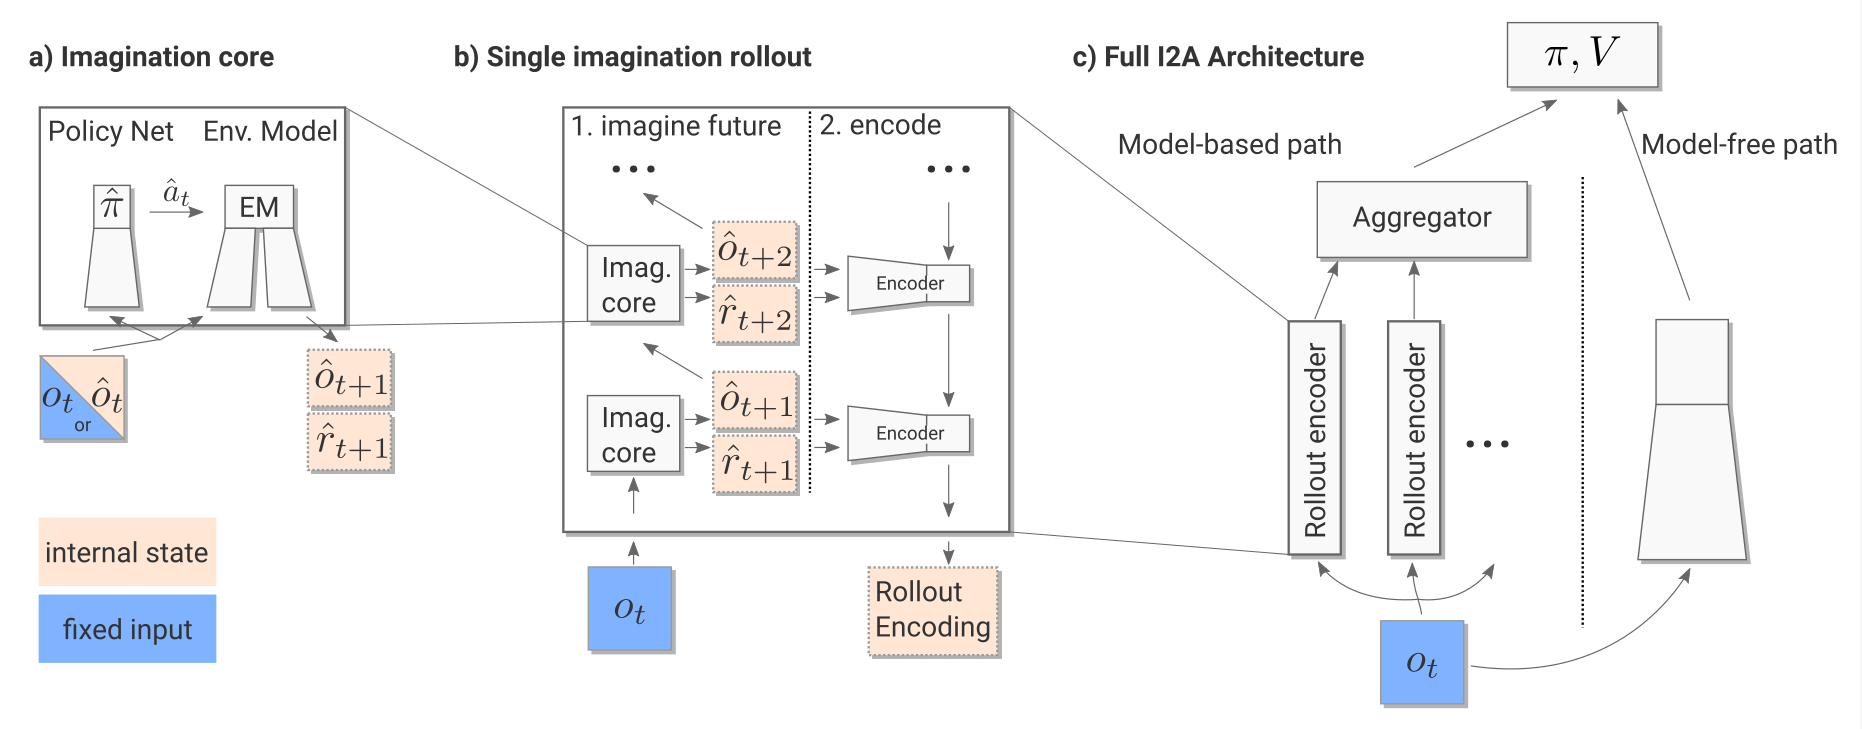
\includegraphics[width=\columnwidth]{./Images/i2a_architecture.png} 
  \caption{Network architecture for deep reinforcement learning which combines model free and model based reinforcement learning. a) imagination core (IC) predicts the next time step conditioned on an action sampled from the rollout policy $\hat{\pi}$. b) the from the imagination core imagines trajectories of features f encoded by the rollout encoder. c) the full i2a} 
  \label{fig:i2a_architecture} 
\end{figure} 
 
\subsection{Imagination core}

The \textbf{imagination core} (Figure \ref{fig:i2a_architecture} a)) imagine the next observation $\hat{o}_{t+1}$ and the next reward $\hat{r}_{t+1}$ given the observation $o_t$ or $\hat{o}_{t}$, where $o_t$ refers to the  input the i2a get and $\hat{o}_{t}$ refers to an internal state of i2a which is an output of a previouse rollout with the imagination core.
To do so the imagination core uses a rollout policy, which predict an action given the current state, and an environment model \ref{sec:env_model}, which predict the next observation and the next reward.\\

%$o_t$: initial observation  $\hat{o}_t$: predicted observation  $\hat{r}_t$: predicted reward Given observation $o_t$ or $\hat{o}_t$ and action $\hat{a}_t$ predict (imagine) the next observation $\hat{o}_{t+1}$ and next reward $\hat{r}_{t+1}$  

%To do so the imagination core uses a rollout policy, which decides the next action $\hat{a}_t$, and an environment model, which predicts the next state and the reward signals from the environment, given an state and a current action.\\


The \textbf{rollout policy $\hat{\pi}$} is a model-free reinforcement learning agent which should, given the same observation, predict the same action as the i2a policy. To ensure this, the rollout policy need to be similar to the i2a policy $\pi$, which can be ensure by minimizing the distillation loss, the cross entropy between the rollout policy $\hat{\pi}$ and the i2a policy $\pi$:

%Distillation loss Make $\hat{\pi}$ (rollout policy) and $\pi$ (i2a policy) similar\\ 
 
\begin{equation} 
    l_{dist}(\pi, \hat{\pi})(o_t) = \lambda_{dist} \sum_a \pi(a | o_t) log \hat{\pi}(a|o_t) 
\end{equation} 

with scaling parameter $\lambda_{dist}$.\\
% $\lambda_{dist}$ is set to 10



\subsection{Environment Model (EM)}
\label{sec:env_model}

The environment model predict (imagine) the next observation $\hat{o}_{t+1}$ and next reward $\hat{r}_{t+1}$, given observation $o_t$ or $\hat{o}_t$ and action $\hat{a}_t$.\\

It is a trained environment model which can not be assumed to be perfect, it might sometimes make wrong prediction.\\

   
\begin{figure}[H] 
  \centering 
   
  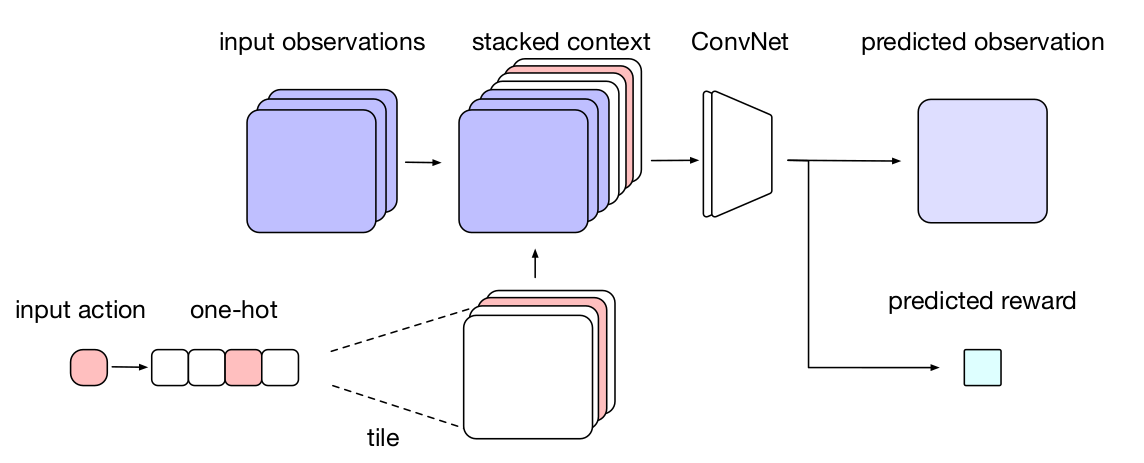
\includegraphics[width=300px]{./Images/environment_model_architecture.png}
  \caption{TODO} 
  \label{fig:environment_model_architecture} 
\end{figure} 

Figure \ref{fig:environment_model_architecture} shows the environment model architecture. It gets as input the last observation as rgb image $o_t$ and the from the rollout policy selected action $a$. The action is converted to a one hot vector and tiled to the size of the observation. The tiled action is then concatinated with the input observations. A convolutional neural network with two heads predicts then the next observation and the expected reward.\\

The neuronal network is trained with pairs of $(o_t, a_t) \rightarrow (o_{t+1}, r_{t+1})$ generated from a pretrained model-free advantage-actor-critic policy. This is nessesary because a random agent is not able to generate a representative set of states, as it sees few rewards in some of the domains.\\

 
The environment model is trained by maximize the log likelihood of the probability $p(o_t | a_{t-1}, o_{t-1})$. Where $p(o_t | a_{t-1}, o_{t-1})$ is a bernoulli distribution: 
\begin{equation} 
   p(o_t | a_{t-1}, o_{t-1}) = x^y (1-x)^{1-y} 
\end{equation} 
   
$log p(o_t | a_{t-1}, o_{t-1})$ equals to Binary Cross Entropy between the true image and the predicted imageloss 
   
\begin{equation} 
  \mathnormal{ 
  env_{loss}(x, y) = \frac{1}{N} \sum y_n log x_n + (1-y_n) log(1- x_n) 
  %env_{loss} = Binary Cross Entropy(predicted\_image, true\_images) 
  } 
  \end{equation} 
 
 
 
\subsection{Single Imagination Rollout}
 
 
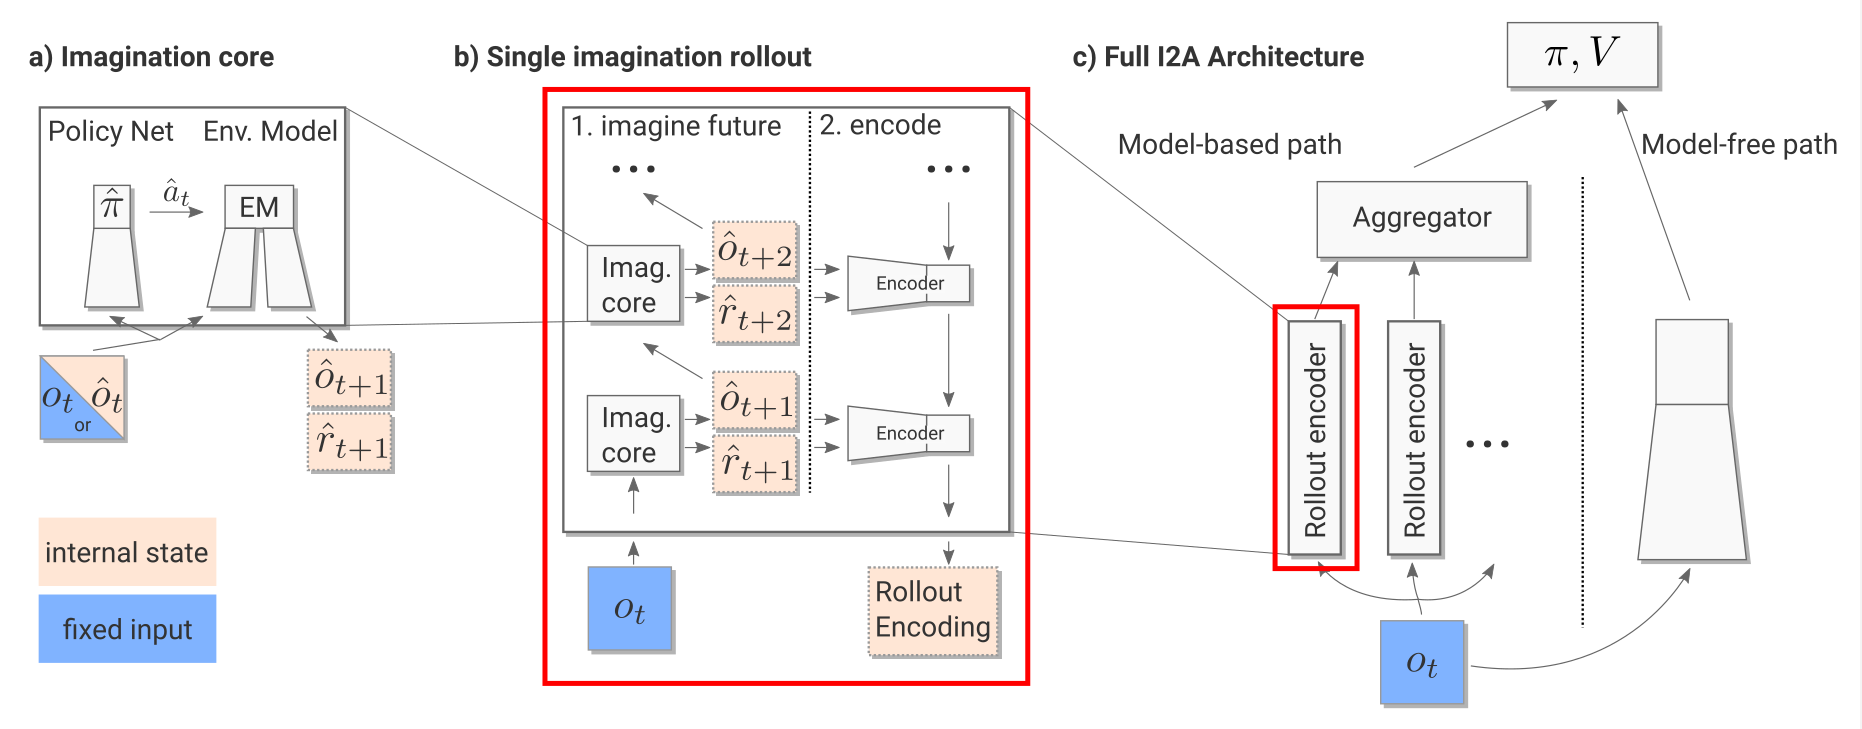
\includegraphics[width=\columnwidth]{./Images/i2a_all_imagination_rollout.png}% 
 
The imagination core imagines trajectories of features $f = (\hat{o}, \hat{r})$\\ 
The rollout encoder encode these trajectories     
 
 
 
I2A Architecture - Imagination Future 
 
Input:\\ 
    observation $o_t$ \\ 
    (1 MiniPacman frame)\\ 
    start action $a$ 
Output:\\ 
    n imagined trajectories ($\hat{o}_{t+i}, \hat{r}_{t+i}$ for $i = 0, ..., n$) 
     $\hat{} \hspace{2mm} \rightarrow$ internal state 
   
  %\begin{center} 
    %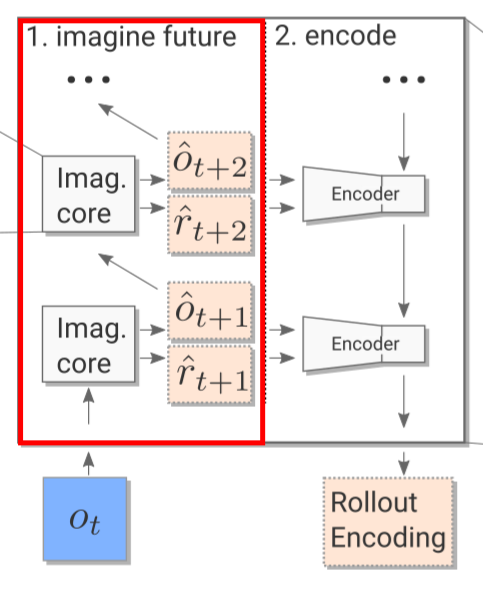
\includegraphics[height=.5\textheight]{./Images/imagine_future.png}% 
  %\end{center} 
 
I2A Architecture - Encoder 
 
     CNN Network followed by an LSTM Network 
    CNN Network:\\ 
    Encode observation and reward $\hat{o}_{t+i}, \hat{r}_{t+i}$ 
    LSTM Network:\\ 
    Learns long-term dependencies 
    %\item Learns useful information from the rollout trajectories 
   
  \begin{center} 
    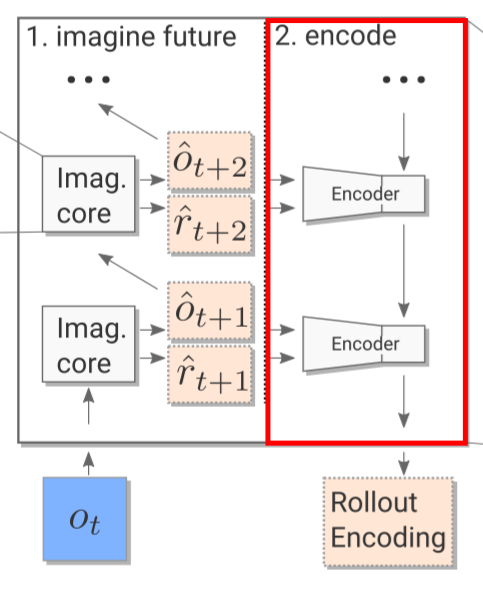
\includegraphics[height=.2\textheight]{./Images/encoder.png}% 
  \end{center} 
 
 
 
I2A Architecture - Model Based Path 
 
 
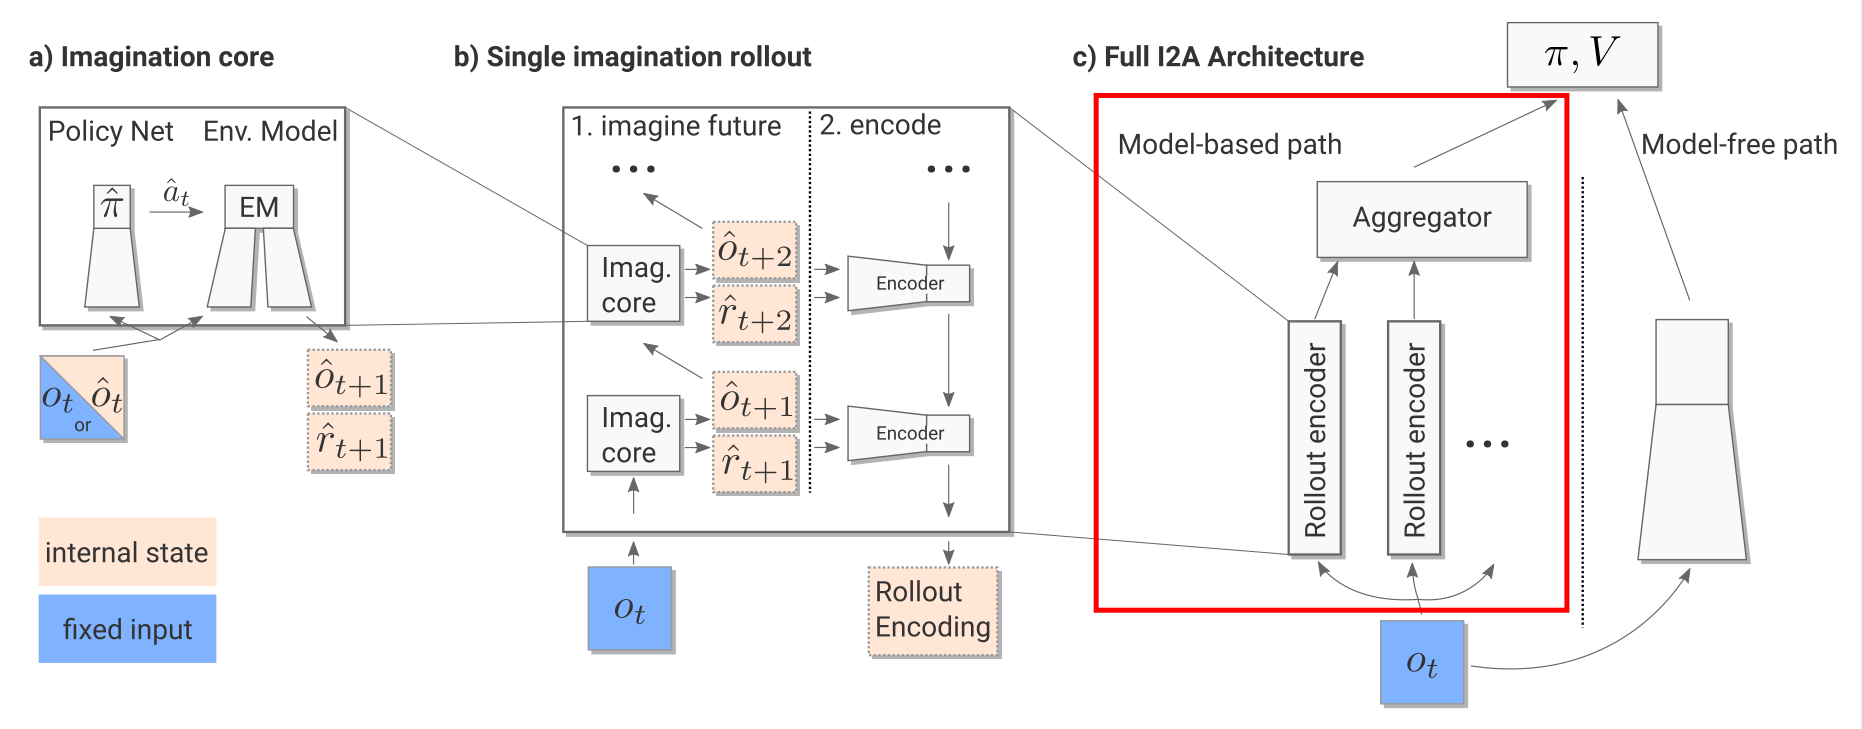
\includegraphics[width=\columnwidth]{./Images/i2a_all_model_based_path.png}% 
 
%For each action $a$ the agent can take do a imagination rollout  
% the future based on a model of the environment and use this information for decision making 
 
 
I2A Architecture - Model Based Path 
 
 
       For each action $a$ the agent can take, do a imagination rollout  
    %For each action the agent can take,  
    %imagine the future% and learn relevent information that can happen 
     Aggregator: \\ 
    Concatinate all action rollouts 
   
  %\begin{center} 
    %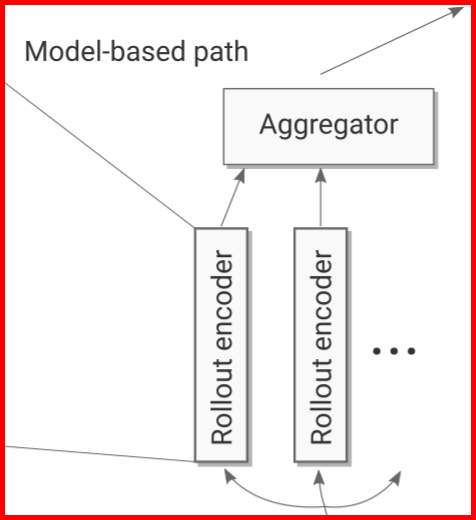
\includegraphics[height=.5\textheight]{./Images/i2a_model_based.png}% 
  %\end{center} 
 
 
 
I2A Architecture - Model Free Path 
 
 
 
CNN Layers followed by Fully Connected Layers 
 
 
 
I2A Training 
Input:\\ 
    Observation $o_t$ 
     Output:\\ 
    Policy $\pi$ and value function $V$ 
     Train with Advantage-Actor-Critic (A2C) 



\section{Environment Model}

 
b






\section{Mini Pacman}


The I2A architecture contains much more weights to learn than a model-free advantage-actor-critic architecture. If  is a very big network compared to the model free 

\begin{figure}[H] 
  \centering   
  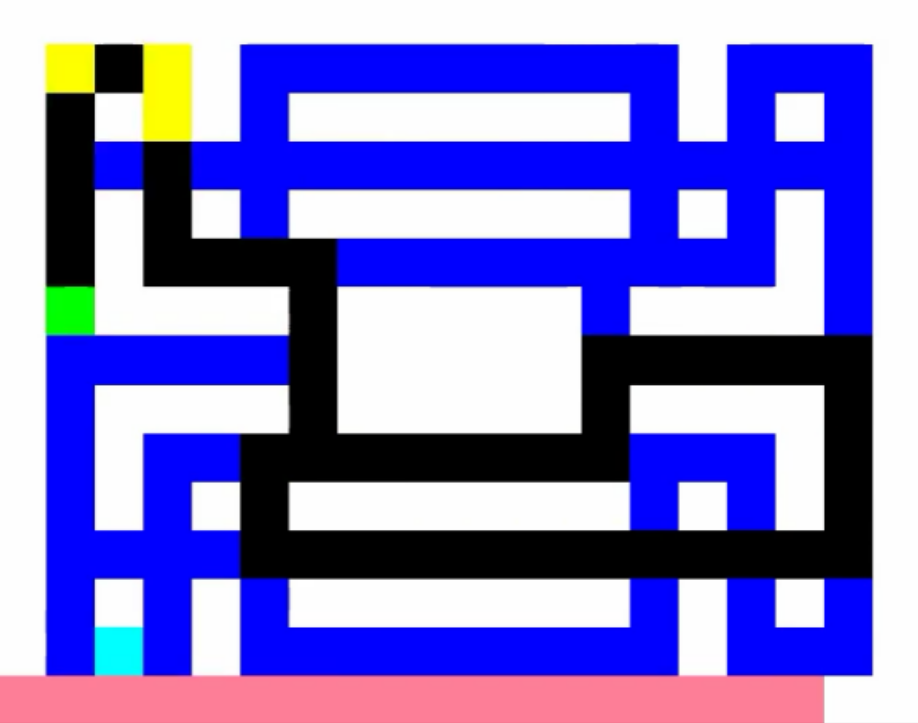
\includegraphics[width=0.5\columnwidth]{./Images/mini_pacman.png}
  \caption{Mini Pacman} 
  \label{fig:environment_model_architecture} 
\end{figure} 


I2A Model Based Path expensive to train
• Uses 15 x 19 Grid World version of Pacman
• Makes vision problem easier but preserves the reinforcement
learning problem
•
MiniPacman can be played in different modes



Hunt Rewards:\\

\begin{center}
	\begin{tabular}{ p{4cm}  r }
 	At each step & 0 \\
  	Eating food & 0 \\
	Eating power pill & 1\\
	Eating ghost & 10\\
	Killed by ghost & -20\\
	\end{tabular}
\end{center}

\section{Results}

This section shows the results of the environment model and the i2a implementation. Also it shows the performance of i2a over the model-free baseline and the copy model.

%In the following the performance of I2A over the model-free baseline and the copy model is shown. Also the predicted rollouts of the environment model.

\subsection{Environment Model Training}

Our trained environment model is an imperfect model, which is in most cases able to predict a few steps into the future, but it is bad at predicting far into the future.\\





\begin{figure}[H] 
  \centering   
  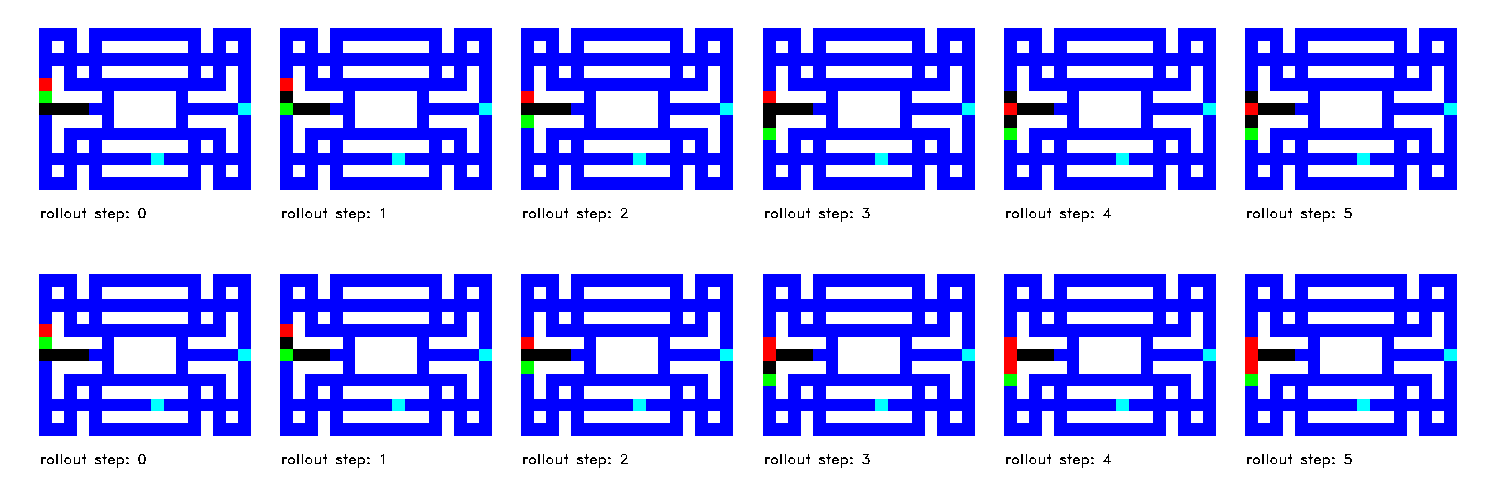
\includegraphics[width=\columnwidth]{./Images/env_model_rollouts.png}
  \caption{Environment model rollouts, top true observations, bottom predicted observations, rollout steps from left to right} 
  \label{fig:environment_model_rollouts} 
\end{figure} 



Figure \ref{fig:environment_model_rollouts} shows the true next observations in the upper row and the predicted next observations in the lower row. From left to right it shows the rollout steps, the prediction is always based on the previous rollout step. In the beginning the prediction is quite good but the errors accumulate, leading to prediction errors like the one in rollout step 3 of figure \ref{fig:environment_model_rollouts}. The environment model is unsure where the ghost, the red points, are moving and as a result it predicts the ghost at two positions.\\



TODO check numbers\\
The environment model was trained for 2000 million frames, on a Titan Xp GPU for ~160 hours with around 3470 frames per second. As optimizer we used Adam with a learning rate of $10^{-4}$ and a weight decay of 0.01. The batch size was 500 and we weighted the reward loss with a coefficient of 0.01 compared to the frame loss. To train the environment model with a representative set of observations, we used as described in section \ref{sec:env_model} a pretrained a2c policy to create samples of pairs of observation and reward.
%1352.8min + 8274.3
% main_train_environment_model.py --env-name HuntMiniPacmanNoFrameskip-v0 --environment-model MiniModel --lr 1e-4 --save-interval 100 --batch-size 500 --sample-memory-size 1500 --num-episodes 300000000 --port 5028

\begin{figure}[H] 
  \centering   
  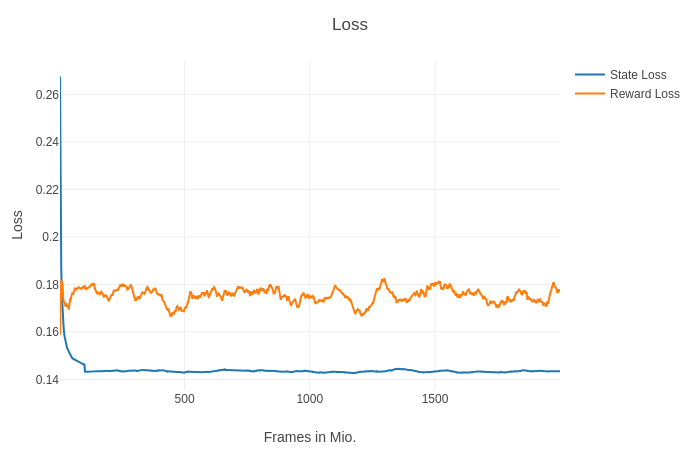
\includegraphics[width=0.7\columnwidth]{./Images/hunt_env_loss_curve.png}
  \caption{Environment model loss curve} 
  \label{fig:env_model_loss} 
\end{figure} 

The figure \ref{fig:env_model_loss} shows the loss curve of the environment model training. It seems as if the loss stagnates very soon, but the main advantage in correct predictions is learned in the part with small loss changes. To learn the general structure of the maze is easy but to predict the correct position of the player and the ghosts is really hard, but has only a small impact on the loss.\\




\subsection{I2A MiniPacman Results}

In this section we demonstrate the performance of our reinforcement learning agent and compare our results with the results of the "imagination augmented agent for deep reinforcement learning" paper \cite{I2A}.
%In this section we compare the performance of our reinforcement learning agent to the results of the paper.
To do so we trained three different agents, an a2c model-free baseline, the copy model and the i2a agent on the reinforcement learning task MiniPacman in the modes "Regular" and "Hunt".\\
%To do so we trained MiniPacman in the mode 'Regular' and 'Hunt' with 3 different agents, a A2C model-free baseline, the copy model and the I2A agent.
%To compare the performance, we trained MiniPacman Hunt with a A2C model-free baseline, the copy model and I2A agent.\\

As baseline for our implementation we used the a2c reinforcement learning pytorch implementation of Ilya Kostrikov\cite{pytorchrl}.

%\begin{comment}
\begin{figure}[H] 
    \centering
    \begin{subfigure}[b]{0.45\textwidth}
        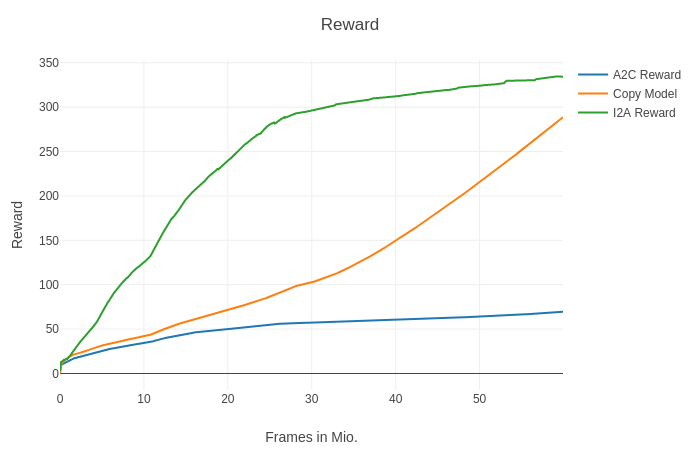
\includegraphics[width=\textwidth]{./Images/regular_rewards_compare.png}
  		\caption{Received reward of i2a run with 2 rollouts (green), model-free a2c baseline (blue) and copy model (orange).} 
  		\label{fig:mini_pacman_regular_rewards} 
    \end{subfigure}
	~ %add desired spacing between images, e. g. ~, \quad, \qquad, \hfill etc.       
    \begin{subfigure}[b]{0.45\textwidth}
        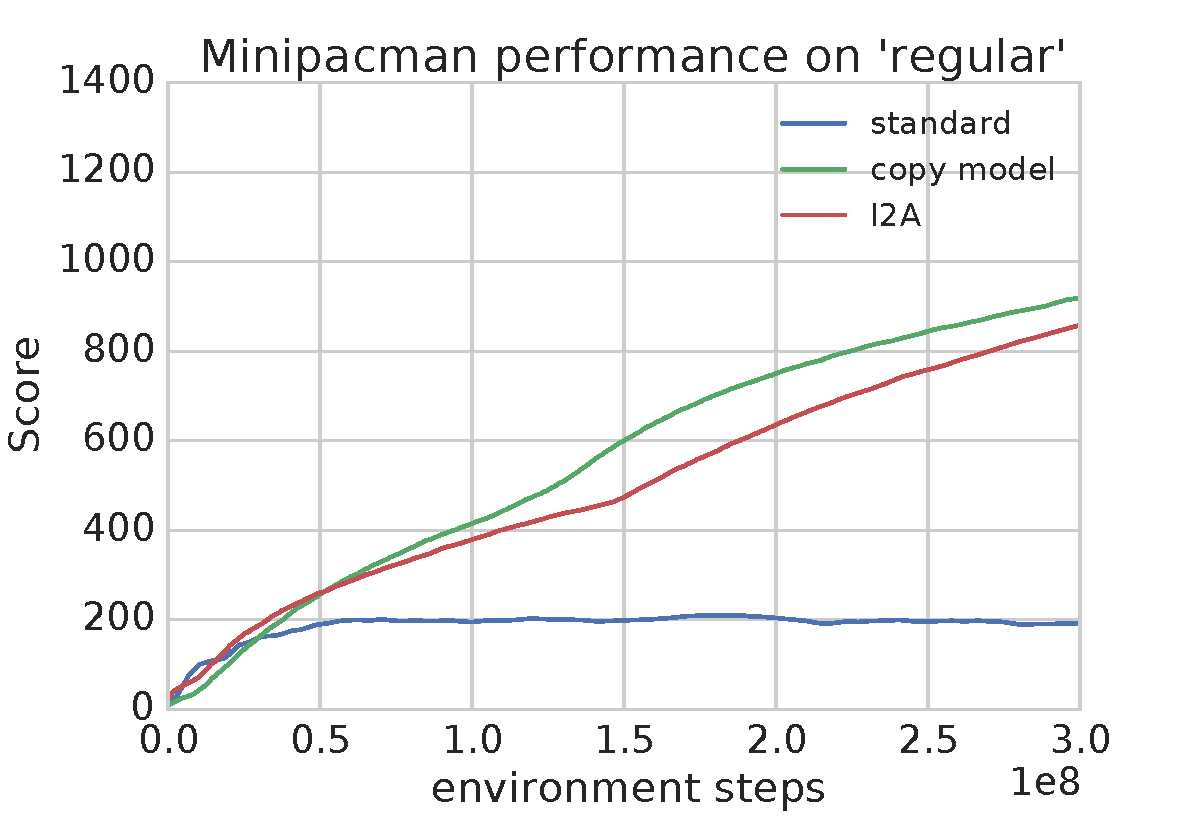
\includegraphics[width=\textwidth]{./Images/minipacman_regular.pdf}
  		\caption{Received rewards from the "imagination augmented agent for deep reinforcement learning" paper \cite{I2A}.} 
  		\label{fig:mini_pacman_regular_original_rewards}
    \end{subfigure}
    
    \caption{Learning curves for different agents on the task MiniPacman Regular}\label{fig:mini_pacman_regular}
\end{figure}

%\end{comment}

Figure \ref{fig:mini_pacman_regular_rewards} shows our training results for the reinforcement learning task MiniPacman Regular. The a2c baseline is clearly outperformed by the copy model and the i2a model, but there is no performance improvement of the i2a over the copy model. The performance improvement therefore only corresponds to the parameter increasement and not to the imagined rollouts. 
Our results match with the results of the original i2a paper which also have no improvement of i2a over the copy model in the mode "Regular" as shown in figure \ref{fig:mini_pacman_regular_original_rewards}.
We trained our agents for 100 million frames on a Titan Xp which took for the a2c baseline $\sim$16 hours, for the copy model $\sim$36 hours and for the i2a $\sim$63 hours.


\begin{figure}[H] 
    \centering
    \begin{subfigure}[b]{0.45\textwidth}
        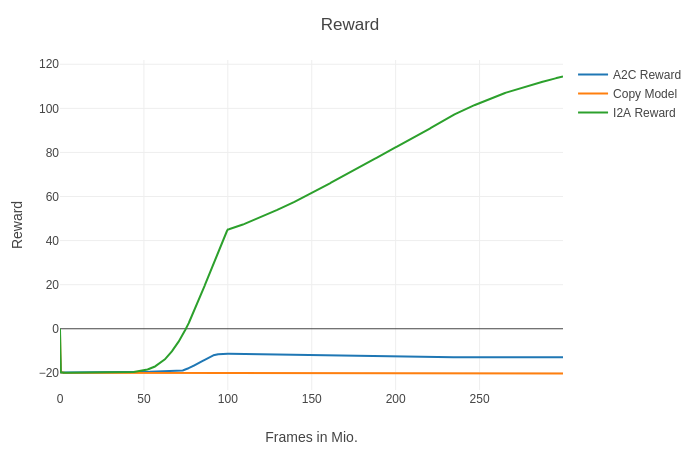
\includegraphics[width=\textwidth]{./Images/hunt_rewards_compare.png}
  		\caption{Received reward of I2A run with 2 rollouts (green), model-free A2C baseline (blue) and copy model (orange).} 
  		\label{fig:mini_pacman_hunt_rewards} 
    \end{subfigure}
	~ %add desired spacing between images, e. g. ~, \quad, \qquad, \hfill etc.       
    \begin{subfigure}[b]{0.45\textwidth}
         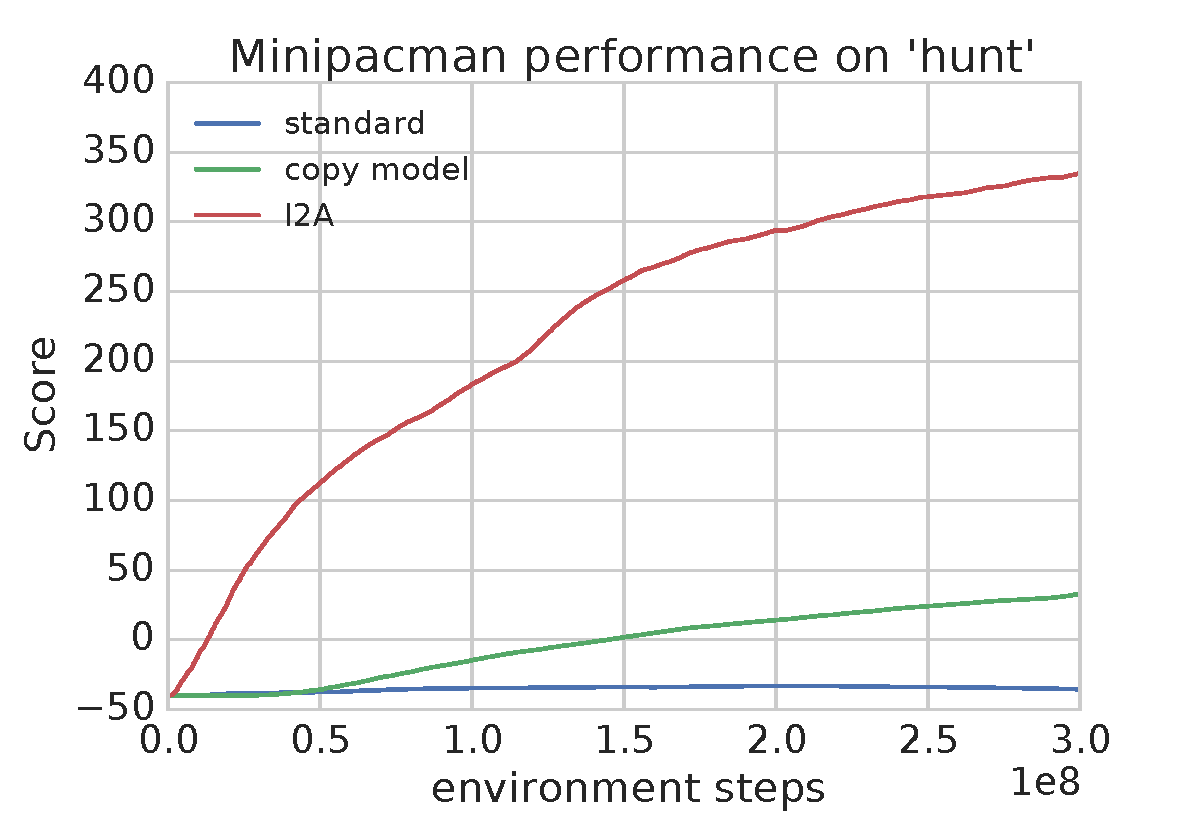
\includegraphics[width=\textwidth]{./Images/minipacman_ghosthunt.pdf}
		 \caption{Received rewards from the "imagination augmented agent for deep reinforcement learning" paper \cite{I2A}.} 
		\label{fig:mini_pacman_hunt_original_rewards} 
    \end{subfigure}
    
    \caption{Learning curves for different agents on the task MiniPacman Hunt}\label{fig:mini_pacman_hunt}
\end{figure}

The results of the trained agents on MiniPacman in Hunt mode are shown in figure \ref{fig:mini_pacman_hunt}. As you can see i2a outperforms clearly the a2c baseline and the copy model shown in figure \ref{fig:mini_pacman_hunt_rewards}.
As before our results match the ones from the paper, see figure \ref{fig:mini_pacman_hunt_original_rewards}, only the maximum reward we reached with our i2a agent is not as high as the results of the original paper.
This difference could be caused by the fact that they use a rollout length of 5 and we only a rollout length of 2.
We trained MiniPacman Hunt for 300 million frames on a Titan Xp  which took for the a2c baseline $\sim$48 hours, for the copy model $\sim$94 hours and for the i2a $\sim$215 hours.\\ 
%A possible reason for this difference is that they use in the paper a rollout lenght of 5 and we use only a rollout length of 2.


The reproduced results from the paper support the statement that the performance gap between i2a and baselines is high for tasks where the rewards are sparse and where planning ahead is important to avoid irreversible actions, as for example move pacman to a position where he gets enclosed by ghosts.
%Hunt due to it's sparse reward and the increasing number of ghosts is a more planning related problem as MiniPacman in Regular mode.



%main.py --algo i2a --env HuntMiniPacmanNoFrameskip-v0 --num-processes 128 --port 5555 --log-dir /tmp/gym/Hunt_AfterBugfix --num-steps 10 --entropy-coef 0.02 --distill-coef 0.3 --num-stack 1 --use-class-labels
%TODO compare result with the one of the i2a paper.



\begin{comment}
\begin{figure}[H] 
  \centering   
  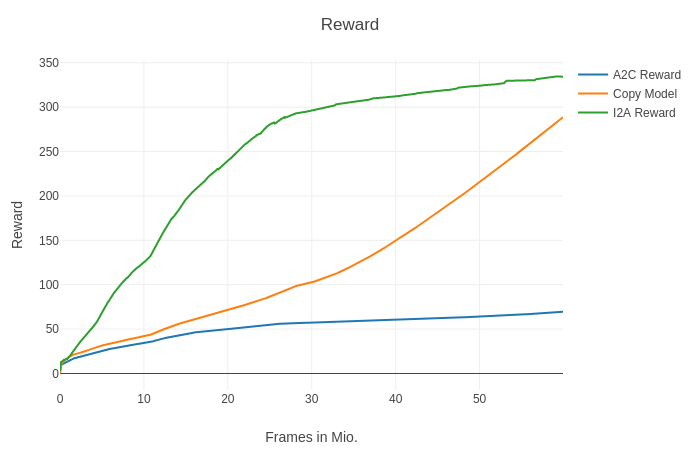
\includegraphics[width=0.7\columnwidth]{./Images/regular_rewards_compare.png}
  \caption{Reached rewards on the environment MiniPacman Hunt. Green curve I2A run with 2 rollouts, blue curve model-free A2C baseline and orange curve copy model results.} 
  \label{fig:mini_pacman_regular_rewards} 
\end{figure} 


\begin{figure}[H] 
  \centering   
  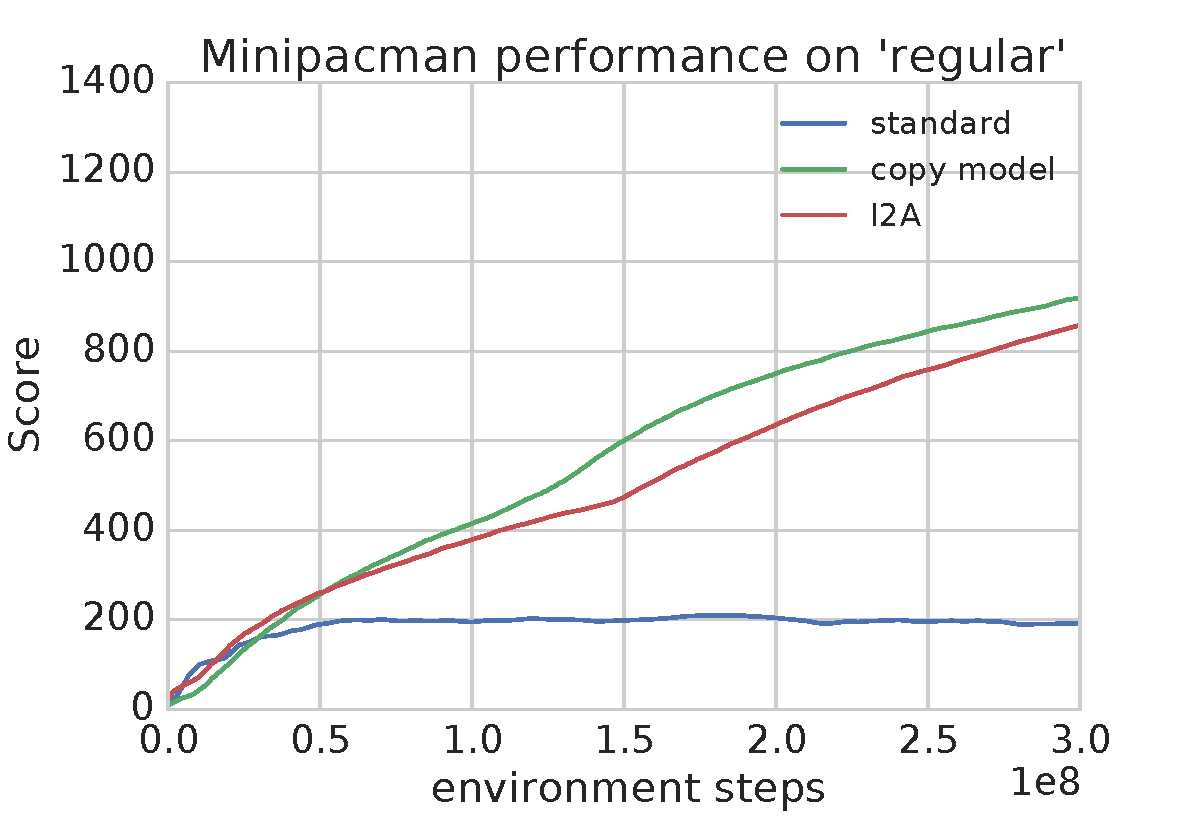
\includegraphics[width=0.7\columnwidth]{./Images/minipacman_regular.pdf}
  \caption{Results from the paper} 
  \label{fig:mini_pacman_regular_original_rewards} 
\end{figure} 
\end{comment}

\begin{comment}
\begin{figure}[H] 
  \centering   
  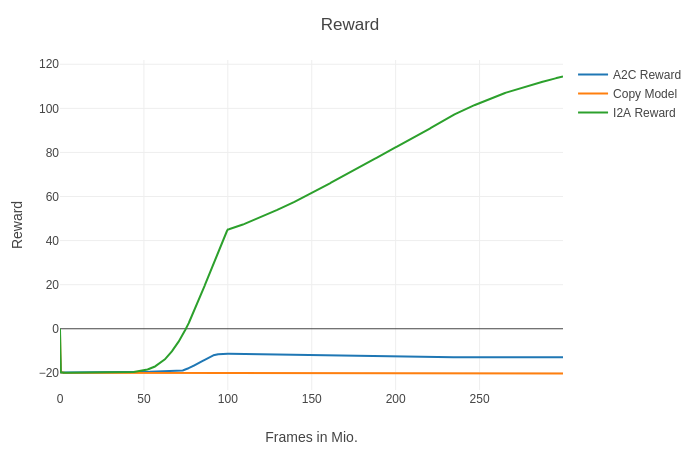
\includegraphics[width=0.9\columnwidth]{./Images/hunt_rewards_compare.png}
  \caption{Reached rewards on the environment MiniPacman Hunt. Green curve I2A run with 2 rollouts, blue curve model-free A2C baseline and orange curve copy model results.} 
  \label{fig:mini_pacman_hunt_rewards} 
\end{figure} 

\begin{figure}[H] 
  \centering   
  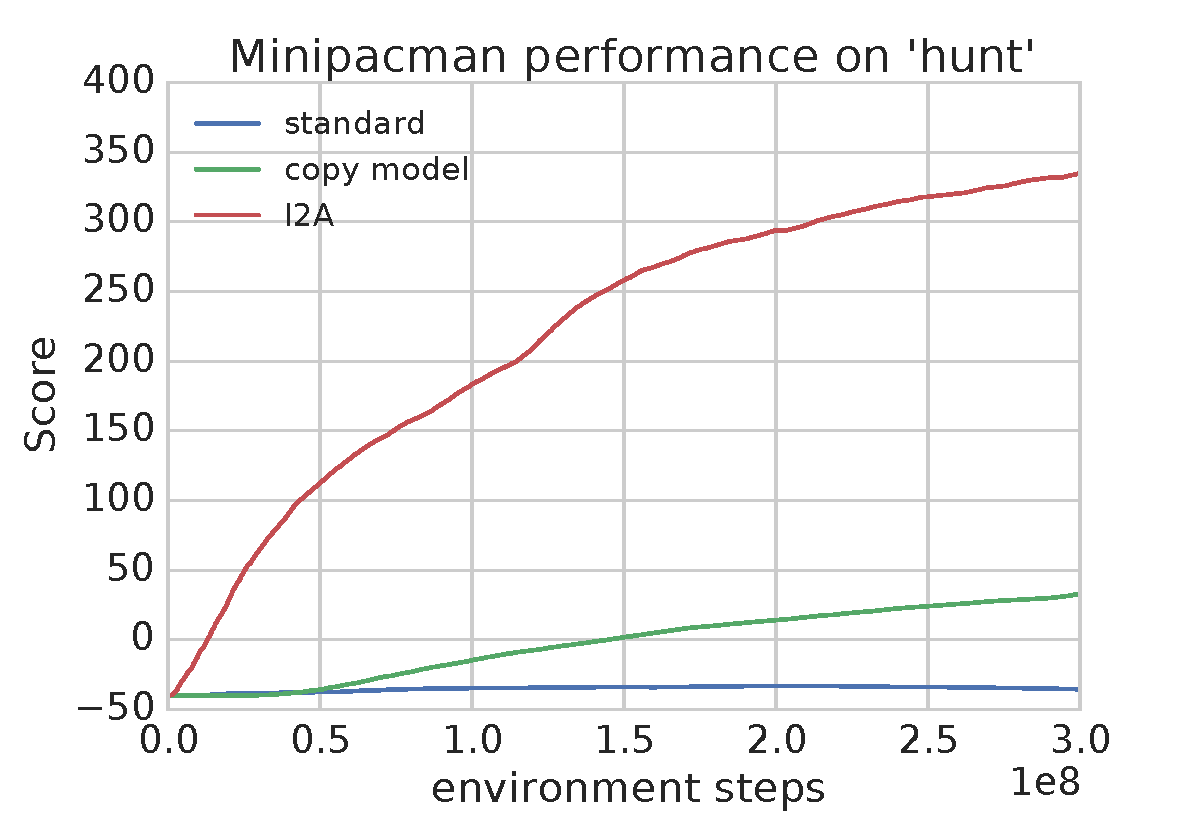
\includegraphics[width=0.9\columnwidth]{./Images/minipacman_ghosthunt.pdf}
  \caption{Reached rewards on the environment MiniPacman Hunt. Green curve I2A run with 2 rollouts, blue curve model-free A2C baseline and orange curve copy model results.} 
  \label{fig:mini_pacman_hunt_original_rewards} 
\end{figure} 
\end{comment}

\section{Future Work}


...

\vspace*{0.3cm}
..





%+++ Literaturverzeichnis +++++++++++++++++++++++++++++++++++++++++++++++++++++
\renewcommand{\bibname}{Literaturverzeichnis}
\bibliography{verzeichnis1}{}
\bibliographystyle{plain}
%\bibliographystyle{alpha}

%+++ Bilderverzeichnis ++++++++++++++++++++++++++++++++++++++++++++++++++++++++
%\renewcommand\listfigurename{Bilderverzeichnis}
%\listoffigures


\end{document}
